\documentclass{article}

\usepackage[margin=0mm, paperwidth=50.1mm, paperheight=98mm]{geometry}

\usepackage{amsmath}
\usepackage{tikz}
\usetikzlibrary{bayesnet}
\usepackage{bm}
\providecommand{\mathbold}[1]{\bm{#1}}
\newcommand{\vct}[1]{\mathbold{#1}}

\begin{document}
\thispagestyle{empty}

\begin{center}
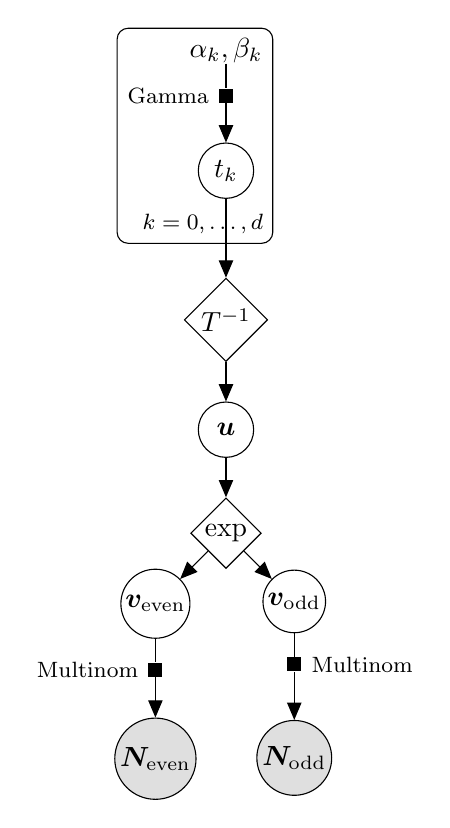
\begin{tikzpicture}
   \node[latent] (t) {$t_k$} ;
   \node[const, above=1 of t] (alpbet) {$\alpha_k,\beta_k$} ;
   \factor[above=.5 of t] {alpbet-t} {left:Gamma} {alpbet} {t} ;
   \plate {alpbett} {(alpbet)(t)} {\rule{2mm}{0mm}$k=0,\ldots,d$} ;
   
   \node[det, below=1 of t] (Tinv) {$T^{-1}$} ;
   \node[latent, below=.5 of Tinv] (u) {$\vct u$} ;
   \node[det, below=.5 of u] (exp) {$\exp$} ;
   \node[latent, below left=.5 of exp] (veven) {$\vct{v}_{\text{even}}$} ;
   \node[latent, below right=.5 of exp] (vodd) {$\vct{v}_{\text{odd}}$} ;
   \node[obs, below=1 of veven] (Neven) {$\vct{N}_{\text{even}}$} ;
   \node[obs, below=1.1 of vodd] (Nodd) {$\vct{N}_{\text{odd}}$} ;
   \edge[->] {t} {Tinv} ;
   \edge[->] {Tinv} {u} ;
   \edge[->] {u} {exp} ;
   \edge[->] {exp} {veven,vodd} ;
   \factor[below=.3 of veven] {veven-Neven} {left:Multinom} {veven} {Neven} ;
   \factor[below=.3 of vodd] {vodd-Nodd} {right:Multinom} {vodd} {Nodd} ;
\end{tikzpicture}
\end{center}

\end{document}











